\begin{figure}[htb!]
  \begin{center}
    \resizebox{\textwidth}{!}{
      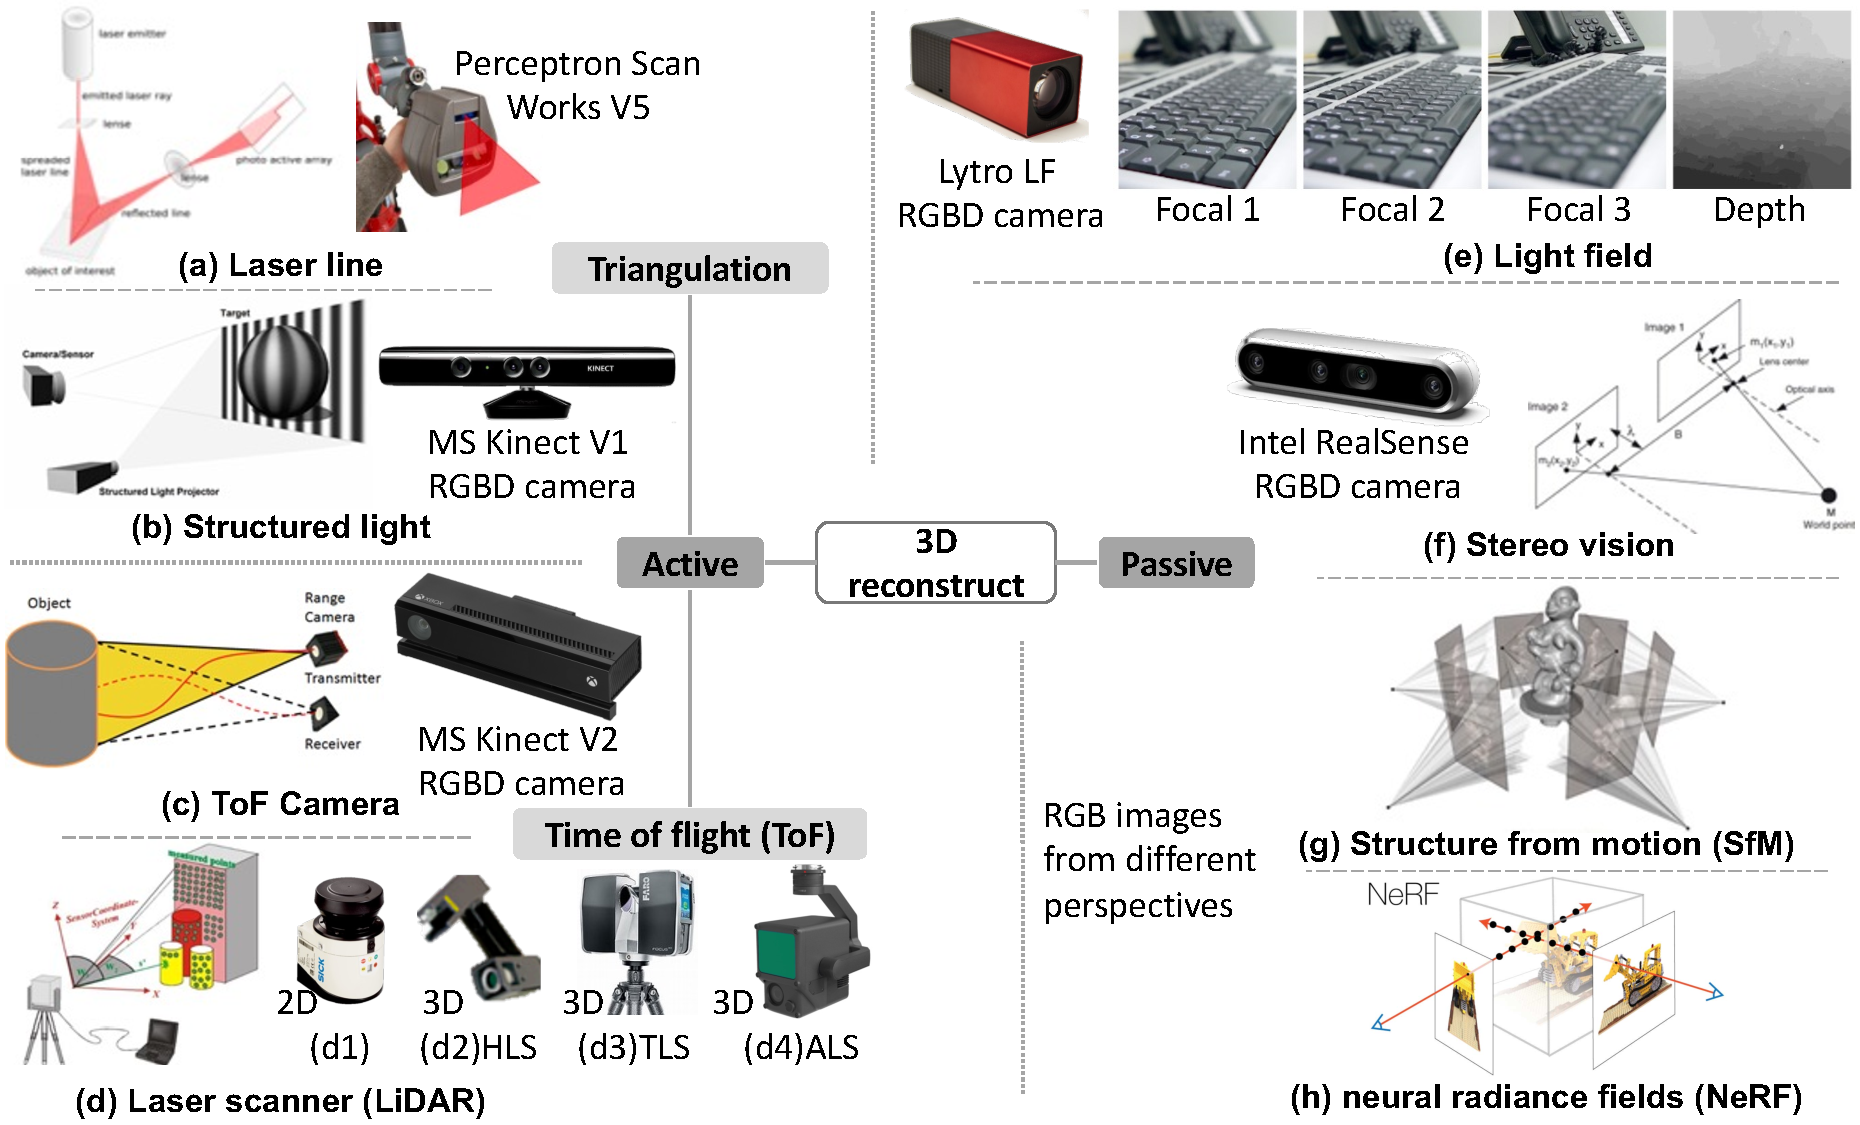
\includegraphics{figures/int/recons_sensors.pdf}
    }
  \end{center}
  \caption[Common approaches for 3D structure reconstruction]{
    Common approaches for 3D structure reconstruction. (a-d) The active sensors rely on projecting lights on the object and analyzing the reflection results, where (d) \acrfull{lidar}; (d2) \acrfull{hls}; (d3) \acrfull{tls}; (d4) \acrfull{als}; (e-f) the passive sensors rely on analyzing the passively received image groups. (e) is a part image of \citep[Fig.~6]{schima_imagine_2016}; (g-h) the \gls{rgb}-based 3D reconstruction algorithms from several perspective images, via (g) conventional geometric deduction and (h) deep learning.
  }
  \label{fig:int2}
\end{figure}